\begin{figure*}[htb!]

\begin{minipage}{0.45\textwidth}

\includegraphics[width=1\linewidth]{../surge/plots/GEV_pi_plateau_NO.pdf}
\caption{First attempt at enforcing a GP asymptote of 2m for New Orleans,
with an \texttt{RBF} kernel.
The data is the same as in Figure~\ref{fig:gev-no}. The
kink is caused by using a non-differentiable mapping to
enforce the far-field conditions. 1$\sigma$ and 2$\sigma$ envelopes shown.}
\end{minipage}
\begin{minipage}{0.45\textwidth}

    \centering
    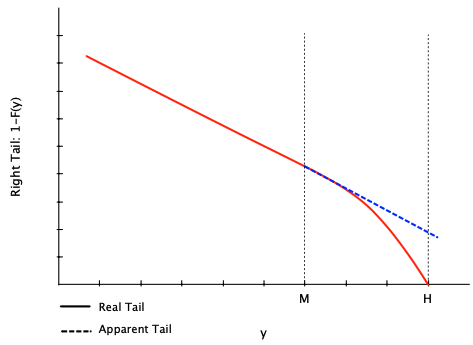
\includegraphics[width=1\linewidth]{images/taleb-limit-slimmed.png}\\
    \textit{Figure 15.1 from T19~\cite{taleb2019statistical} p.~279}
   \caption{As shown if you only
   observe a distribution up to some value M,
    you may be tempted to fit a line through the
   data (dotted blue line).
   But if there were in fact a limit to the distribution at H,
   you would be overestimating
   the true number of very extreme events (red curve),
   predicting events that were larger than were possible.}
   \label{fig:up-bound-taleb}
   \end{minipage}

   \begin{minipage}{0.45\textwidth}
   \centering
   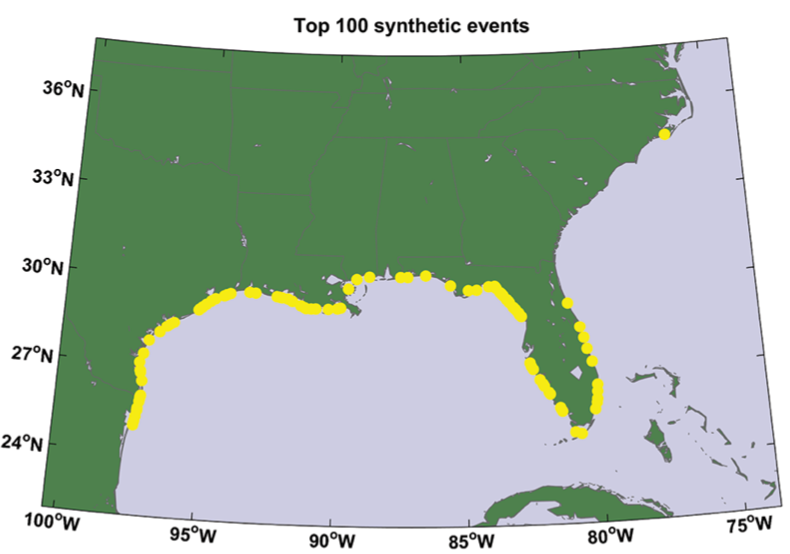
\includegraphics[width=1\linewidth]{images/top-100-landfalls.png}\\
   \textit{Figure 3b from \cite{emanuel2017will}}
   \caption{The top 100 most rapidly intensifying events in the model,
   showing that models capture far more of these TCs in the Gulf of Mexico
   and Florida than further north.
     }
   \label{fig:top-100}
   \end{minipage}
   \begin{minipage}{0.45\textwidth}
   \centering
   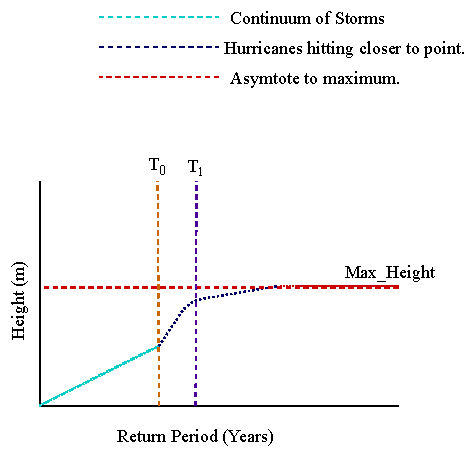
\includegraphics[width=1\linewidth]{images/Return_Hypothesis.pdf}
   \vspace{-15pt}
  \caption{The maximum height is a function of the potential intensity
  allowed by the climate, and the responsiveness of that point on the coastline to a
  wind stress of that size. If T$_0$, or T$_1$, is a similar or greater than the time period of
  measurement, then it is respectively possible that no hurricanes exist in the data sample,
  or that no hurricanes make direct landfall at that location.}
    \label{fig:return_hyp_new}
    \end{minipage}





\end{figure*}
